\documentclass[11pt,letterpaper]{article}

\usepackage[T1]{fontenc}
\usepackage[utf8]{inputenc}
\usepackage[spanish,es-tabla,es-noshorthands]{babel}
\usepackage{lmodern}
\usepackage[margin=2.5cm,headheight=14pt]{geometry}
\usepackage{xcolor}
\usepackage{graphicx}
\usepackage{booktabs}
\usepackage{array}
\usepackage{amsmath}
\usepackage{fancyhdr}
\usepackage{titlesec}
\usepackage[labelfont={bf,color=verde},font=small]{caption}
\usepackage{subcaption}
\usepackage{enumitem}
\usepackage[colorlinks=true,linkcolor=verde,urlcolor=verde,citecolor=verde,
            pdftitle={Auditoria de una STN para el pronostico horario de PM2.5 en Fontibon}]{hyperref}

\definecolor{verde}{HTML}{0B5A43}
\definecolor{dorado}{HTML}{B09A5B}
\definecolor{gris}{HTML}{52514E}

\newcommand{\PM}{PM$_{2,5}$}
\newcommand{\ugm}{\,$\mu$g/m$^3$}

\titleformat{\section}{\Large\bfseries\color{verde}}{\thesection.}{0.6em}{}
\titleformat{\subsection}{\large\bfseries\color{verde}}{\thesubsection.}{0.6em}{}
\titlespacing*{\section}{0pt}{1.2em}{0.6em}
\titlespacing*{\subsection}{0pt}{0.9em}{0.4em}

\pagestyle{fancy}
\fancyhf{}
\fancyhead[L]{\small\bfseries\color{verde}UNIVERSIDAD EXTERNADO DE COLOMBIA}
\fancyhead[R]{\small\color{gris}Deep Learning $\cdot$ Entrega final}
\fancyfoot[L]{\small\color{gris}STN $\cdot$ Beijing $\rightarrow$ Fontibón}
\fancyfoot[R]{\small\thepage}
\renewcommand{\headrulewidth}{0.4pt}
\renewcommand{\footrulewidth}{0.4pt}

\setlist{itemsep=2pt,topsep=4pt}
\setlength{\parskip}{0.45em}
\setlength{\parindent}{0pt}

\begin{document}

% ------------------------------------------------------------------ portada
\begin{titlepage}
\centering
{\color{verde}\rule{\textwidth}{2pt}}\par\vspace{2.2cm}
{\Large\bfseries\color{verde} UNIVERSIDAD EXTERNADO DE COLOMBIA}\par\vspace{0.3cm}
{\large Facultad de Ciencia de Datos}\par\vspace{2.2cm}
{\large Proyecto Integrador de Deep Learning}\par\vspace{0.3cm}
{\large\bfseries ENTREGA FINAL}\par\vspace{1.4cm}
{\huge\bfseries\color{verde} Auditoría de una red Transformer\\[0.2cm] con atención dispersa}\par\vspace{0.4cm}
{\Large para el pronóstico horario de \PM}\par\vspace{0.3cm}
{\large\color{gris} De Beijing a la estación Fontibón (Bogotá)}\par\vspace{1.0cm}
{\color{dorado}\rule{0.6\textwidth}{1pt}}\par\vspace{1.6cm}
\begin{tabular}{rl}
\textbf{Integrante:} & Johan Velandia\\
\textbf{Docente:} & Wilmer Darío Pineda Ríos\\
\textbf{Asignatura:} & Deep Learning
\end{tabular}\par
\vfill
{\large Bogotá, D.\,C. $\cdot$ 2026}\par\vspace{0.4cm}
{\color{verde}\rule{\textwidth}{2pt}}
\end{titlepage}

% ------------------------------------------------------------------ cuerpo
\section{Modelo final y consolidación del traslado}

La pregunta del proyecto es si una \emph{Sparse Attention-based Transformer Network} (STN) [1], que adapta la atención ProbSparse de
Informer [4] a la arquitectura Transformer [5], replicada en Beijing [3] y trasladada a la estación Fontibón, pronostica mejor el \PM{} de la hora siguiente que una
regresión Ridge, y si el preentrenamiento en Beijing ayuda. En la Fase 2 se compararon tres estrategias en
validación: entrenamiento desde cero (A), extractor congelado (B) y ajuste parcial del decoder (C).

\textbf{Selección.} El modelo final es \textbf{A}. Se eligió con el criterio fijado en la Primera Entrega,
menor RMSE medio de validación (A 6,314; C 6,627; B 6,834\ugm), y mostró baja variabilidad entre semillas
(DE = 0,061). Aunque C presentó menor dispersión (0,040), su RMSE fue superior; B mostró una dispersión
menor (0,016), pero solo contó con dos corridas completas. Por ello, el criterio principal predefinido de
RMSE favoreció a A. C entrenó más rápido (1,2–1,9\,h frente a 2,4–3,5\,h), pero eso no compensa su
mayor error. D y la tercera semilla de B no se completaron y quedan como limitaciones declaradas.

\textbf{Protocolo.} Antes de evaluar el conjunto de prueba y calcular cualquier métrica sobre él, se dejó por escrito el modelo final, las
semillas, las métricas, el umbral de episodio alto (40\ugm) y los criterios de decisión,
incluyendo el SHA-256 de cada checkpoint. Antes de calcular cualquier métrica de prueba, los ocho
checkpoints reprodujeron exactamente su RMSE de validación de la Fase 2, y Ridge, reajustado como en la
Fase 1, reprodujo su RMSE de prueba (7,063). La evaluación se ejecutó una sola vez, por inferencia y sin
entrenamiento.

\begin{table}[h]
\centering
\caption{Fontibón, prueba (2.574 ventanas, 14-sep a 31-dic de 2022). Media $\pm$ desviación muestral entre semillas.}
\small
\begin{tabular}{lcccccc}
\toprule
Modelo & Semillas & RMSE & MAE & $R^2$ & RMSE ($\geq$40) & Sesgo ($\geq$40)\\
\midrule
\textbf{A: desde cero} & 3 & \textbf{6,869 $\pm$ 0,020} & 4,969 & 0,616 & 17,25 & $-$13,95\\
C: ajuste parcial & 3 & 7,274 $\pm$ 0,038 & 5,294 & 0,569 & 18,77 & $-$15,73\\
B: congelado & 2 & 7,484 $\pm$ 0,051 & 5,429 & 0,544 & 19,52 & $-$16,70\\
Ridge (línea base) & -- & 7,063 & 5,115 & 0,593 & 17,87 & $-$14,96\\
Persistencia & -- & 8,232 & 5,843 & 0,448 & 16,66 & $-$9,80\\
\bottomrule
\end{tabular}
\end{table}

A reduce el RMSE de Ridge en 0,19\ugm{} (2,7\,\%) en las tres semillas. El intervalo bootstrap del 95\,\%
con bloques móviles de 24 horas excluye el cero en todas, con extremos entre $-0{,}34$ y $-0{,}05$. La
mejora es real pero pequeña: A comete menos error que Ridge solo en el 51–53\,\% de las ventanas.
B y C quedan por encima de A en cada semilla y también por encima de Ridge, así que la transferencia desde
Beijing no ayudó, igual que en validación (figura~\ref{fig:comp}). La figura~\ref{fig:test} muestra que el modelo sigue bien el
nivel y el ciclo diario, pero llega tarde y corto a los picos.

\textbf{Contraste con el artículo.} Del método se conservaron la arquitectura encoder–decoder con
atención dispersa, la ventana de 24 horas, el horizonte de una hora, la pérdida MSE, Adam con tasa
$10^{-4}$, el escalado MinMax y las métricas. Cambiaron la profundidad (2 encoders y 1 decoder frente a
3 y 2), el número de variables (tres frente a ocho) y la validación (cronológica frente a aleatoria). En
Beijing la réplica obtuvo RMSE 21,13 $\pm$ 0,40 frente a 19,04 del artículo. En Fontibón el RMSE absoluto es numéricamente menor
(6,87), pero no es directamente comparable con Beijing debido, entre otras diferencias, a que los niveles de \PM{} son unas cinco veces más bajos; además, el $R^2$ cae de 0,95 a 0,62. La serie local
es mucho menos persistente (autocorrelación a una hora de 0,74 frente a 0,96) y su variación hora a hora es
más difícil de anticipar con solo \PM, temperatura y punto de rocío. En Taizhou, la segunda serie del
artículo y de niveles comparables, los autores reportan $R^2 = 0{,}924$ con más variables. Aunque no es una
comparación controlada, apunta a la información disponible, más que a la arquitectura, como el límite
principal.

\section{Auditoría mediante explicabilidad}

Se combinaron cuatro evidencias sobre las tres semillas de A: mapas de atención, gradientes integrados
[7], ablaciones sobre la prueba y casos sintéticos de comportamiento esperado. Antes de interpretarlas se
comprobó que fueran fieles. Los mapas se extrajeron con un recorrido manual capa por capa que reproduce la
predicción del modelo (diferencia máxima de $2\times10^{-7}$). Los gradientes integrados cumplen la
propiedad de completitud: las atribuciones suman el cambio de la predicción respecto a la línea base, con
un error medio cercano al 5\,\%.

\textbf{Qué usa la red.} El 70\,\% de la atribución recae en las últimas seis horas y el 24\,\% solo en el
\PM{} de la última hora (figura~\ref{fig:ig}). Por variable, el \PM{} aporta el 46\,\% y la temperatura y
el punto de rocío el 27\,\% cada una; en episodios altos el \PM{} sube al 58\,\%. Las ablaciones confirman
que la red usa toda la entrada:
\begin{itemize}
\item reemplazar la meteorología por su media de entrenamiento aumenta el RMSE en 0,69;
\item aplanar la historia de \PM{} en su último valor lo aumenta en 0,76;
\item desordenar las 24 horas lo aumenta en 4,30.
\end{itemize}
En los casos sintéticos (figura~\ref{fig:sint}), las series constantes se reproducen (10 $\rightarrow$
9,9; 40 $\rightarrow$ 38,8) y un pico de 60\ugm{} ocurrido doce horas antes se ignora (15,6 sobre una base
de 15). La red aprendió una dependencia físicamente razonable, en la que pesan la concentración reciente y
las condiciones meteorológicas recientes.

\textbf{El atajo: persistencia suavizada.} La misma auditoría muestra una estrategia conservadora:
\begin{itemize}
\item La predicción se correlaciona más con la última hora observada (0,90) que con el valor real que debe
  predecir (0,785).
\item Recoge solo el 24\,\% de cada subida y el 40\,\% de cada bajada.
\item Ante un escalón de 15 a 35\ugm{} predice 28,5; ante una rampa hasta 45, predice 32,8; ante un pico de
  60 en la última hora, predice 30,6.
\end{itemize}
El modelo amortigua todo cambio reciente y devuelve la predicción hacia la media. En las comprobaciones
realizadas no se encontró evidencia de que la imputación o el mes expliquen este patrón: las ventanas con
datos imputados tienen un error similar (6,97 frente a 6,78) y el desempeño se mantiene estable entre los
meses observados. La estrategia minimiza el error cuadrático promedio a costa de reaccionar tarde.

\textbf{Matrices de atención.} Se graficaron los pesos reales consulta $\times$ clave de la primera capa del
encoder, la única cuyas posiciones todavía corresponden a horas. Los pesos tienen forma (ventana, 4 cabezas,
12 consultas seleccionadas, 24 claves) y se muestran sin promediar. Los ejemplos se eligieron con reglas
fijas que no dependen del error: un episodio normal (real 16,1\ugm) y uno alto (real 47,5\ugm, predicho
en 18,0), figura~\ref{fig:mat}. Se observa lo siguiente:
\begin{itemize}
\item \emph{Patrón posicional.} En las cuatro cabezas aparecen franjas verticales: casi todas las consultas
  atienden las mismas claves. La cabeza 1 atiende las horas $-20$/$-19$ y la última; la cabeza 3, la última;
  la cabeza 4, las horas $-21$ a $-18$; la cabeza 2 es casi uniforme (entropía normalizada 0,98).
\item \emph{Sin reorganización en los episodios.} Entre episodios normales y altos, la masa de las últimas
  seis horas y la posición media de las claves no cambian con un signo consistente en las tres semillas.
\item \emph{Poca sensibilidad al contenido.} En los casos sintéticos (constante 20, rampa a 45 y pico de 60),
  la predicción cambia de 20,7 a 32,7 y 30,6, pero la masa sobre la última hora apenas pasa de 0,11 a 0,14.
  En estos casos, la asignación parece estar dominada por la posición más que por el contenido.
\item \emph{Inestabilidad entre semillas.} Con métricas y atribuciones casi idénticas, la masa sobre las
  últimas seis horas va de 0,17 a 0,41 según la semilla (figura~\ref{fig:att}), mientras que la atribución
  de esas horas se mantiene entre 0,69 y 0,71.
\end{itemize}

Las tres fuentes responden preguntas distintas. La atención dice \emph{qué posiciones reciben peso}, los
gradientes integrados \emph{qué entradas mueven la salida} y las ablaciones \emph{qué información necesita el
modelo}. Los pesos de atención, por sí solos, no identifican qué usa la red [6] y no se presentan como
explicación causal. En conjunto, la evidencia indica que el modelo usa señal temporal y meteorológica
pertinente, pero con un fuerte comportamiento de persistencia suavizada y regresión hacia la media.

\section{Análisis de fallas}

\begin{table}[h]
\centering
\caption{Error por nivel de \PM{} real en la prueba. Sesgo = predicción $-$ real. A = predicción promedio de las tres semillas.}
\small
\begin{tabular}{lccccc}
\toprule
\PM{} real (\ugm) & $n$ & RMSE A & Sesgo A & RMSE Ridge & RMSE persistencia\\
\midrule
$<$ 10 & 556 & 5,07 & $+$3,41 & 5,71 & 5,36\\
10–20 & 1.018 & 5,33 & $+$1,79 & 5,56 & 7,31\\
20–30 & 640 & 5,81 & $-$1,63 & 5,87 & 8,35\\
30–40 & 242 & 8,95 & $-$5,34 & 8,89 & 10,49\\
$\geq$ 40 & 118 & 17,18 & $-$13,95 & 17,87 & 16,66\\
\bottomrule
\end{tabular}
\end{table}

\textbf{Dónde y cuándo falla.}
\begin{itemize}
\item \emph{Regresión a la media.} El modelo sobreestima en aire limpio y subestima los episodios
  (figuras~\ref{fig:nivel} y~\ref{fig:res}). Ridge presenta el mismo patrón, lo que sugiere una limitación
  compartida por la información disponible (tres variables de una sola estación) y no exclusiva de la STN. La ventaja de A se concentra en niveles bajos
  y medios; entre 30 y 40\ugm{} empata con Ridge.
\item \emph{Subidas.} Cuando el \PM{} sube 5\ugm{} o más en una hora ($n=555$), el RMSE es 10,5 y el sesgo
  $-8{,}2$, frente a un RMSE de 3,9 en horas estables. Entre los veinte peores errores, el 90\,\% son
  subestimaciones durante subidas hacia episodios de 40\ugm{} o más. Se concentran entre las 7 y las 9 de
  la mañana y cerca de la medianoche, que son también las horas de mayor error de todos los modelos
  (figura~\ref{fig:hora}).
\item \emph{Lo que no explica las fallas.} La imputación no cambia el error y el desempeño es estable entre
  septiembre y diciembre.
\end{itemize}
En el contexto de aplicación, esto significa que el modelo falla al inicio de los episodios, que es cuando
una alerta tendría valor: usado como alerta temprana, subestimaría el riesgo.

\textbf{Calibración de la confianza.} Como la red produce un solo número, su confianza se evaluó con
intervalos conformales [8], cuyo ancho es el cuantil del error absoluto en validación. En conjunto cubren
casi lo prometido (77–78\,\% para un nominal de 80\,\% y 87\,\% para 90\,\%), pero esa cifra esconde el
problema. Cubren de más en aire limpio (86\,\% y 93\,\% por debajo de 10\ugm) y colapsan en los episodios
(22\,\% y 33\,\% a partir de 40\ugm). El error crece con el nivel y un intervalo de ancho fijo no lo
refleja. La dispersión entre semillas tampoco sirve como medida de confianza: es pequeña (0,9\ugm) y casi
no se relaciona con el error (correlación 0,20).

\textbf{Entradas fuera del dominio.} Para cada ventana de prueba se midió su distancia a la ventana de
entrenamiento más parecida. El error crece con esa novedad: el RMSE es 5,5 en el cuartil más típico y 7,7
en el más novedoso, aunque A supera a Ridge en los cuatro cuartiles. Ninguna concentración real de la
prueba supera el máximo de entrenamiento (79,8 frente a 100,8\ugm). Sin embargo, al introducir 24 horas
constantes de 100, 150 y 200\ugm{} la red predice 69, 70 y 71, y las semillas divergen entre 63 y 87:
\textbf{se satura cerca de 70\ugm} y no podría seguir un episodio extremo.

\section{Dictamen sobre la profundidad}

La guía del curso pide pronunciarse explícitamente sobre este punto [9]. En la Primera Entrega se fijó que la profundidad se justificaría si la STN lograba una reducción
consistente del RMSE frente a Ridge \emph{y} mejoraba el comportamiento en episodios de concentración
elevada.

\begin{enumerate}
\item \textbf{Reducción consistente del RMSE.} Se cumple: las tres semillas quedan por debajo de 7,063 y los
  intervalos bootstrap excluyen el cero. La magnitud es pequeña, 0,19\ugm.
\item \textbf{Mejora en episodios altos.} Se cumple solo formalmente. En la prueba, A obtiene 17,25 frente
  a 17,87, pero en validación no hubo mejora (17,88 frente a 17,85), la persistencia supera a ambos en los
  picos (16,66) y A sigue subestimándolos en unos 14\ugm.
\item \textbf{Costo.} La STN tiene 99.425 parámetros, tarda entre 2,4 y 3,5 horas en entrenar en CPU y unos
  14 segundos en predecir la prueba; Ridge entrena en segundos y predice en 0,002\,s.
\item \textbf{Datos y auditoría.} Con unas 10.800 ventanas de entrenamiento, la red no superó de forma
  apreciable a un modelo lineal con la misma información. Su estrategia aprendida, una persistencia
  suavizada, es algo que un modelo lineal ya captura. La transferencia, pensada para compensar la escasez
  de datos, empeoró el resultado.
\end{enumerate}

\textbf{Dictamen.} Con los criterios pre-registrados, la arquitectura profunda queda justificada
\emph{por un margen estrecho} en el error promedio, pero \textbf{no se justifica para el objetivo que
motivó el proyecto}, que era anticipar mejor los episodios de concentración elevada. Frente a su costo, la
ganancia es pequeña y Ridge sigue siendo una alternativa razonable. La transferencia desde Beijing no se
justifica: B y C fueron peores que A y que la línea base en validación y en prueba.

\section{Limitaciones y proyección}

\textbf{Limitaciones.}
\begin{itemize}
\item \emph{Datos.} Una sola estación y dos años de registros. La prueba cubre solo septiembre–diciembre
  de 2022, no hay viento comparable entre dominios y la correspondencia del archivo institucional con el
  conjunto público de Fontibón [2] no pudo verificarse.
\item \emph{Variable derivada.} El punto de rocío de Fontibón no se midió: se calculó a partir de la
  temperatura y la humedad relativa con la fórmula de Magnus, así que hereda el error de ambas mediciones y
  de la aproximación.
\item \emph{Modelo.} Red reducida, sin búsqueda de hiperparámetros y con un solo horizonte.
\item \emph{Transferencia.} El supuesto de dinámicas compartidas entre Beijing y Fontibón no se sostuvo:
  la semejanza de distribución tras estandarizar no implicaba dinámicas transferibles.
\item \emph{Evaluación.} Tres semillas no permiten inferencia formal y el bootstrap es descriptivo. Los
  intervalos conformales se calibraron con un período distinto (mayo–septiembre). Los gradientes
  integrados dependen de la línea base elegida, y los casos sintéticos fijan la meteorología en su media,
  por lo que también son entradas poco realistas.
\end{itemize}

\textbf{Líneas de continuidad.} Las fallas apuntan a la información y a la pérdida, más que a la
arquitectura. Se propone:
\begin{itemize}
\item incorporar viento, altura de la capa de mezcla y estaciones vecinas;
\item entrenar con pérdidas que castiguen la subestimación (cuantílica o ponderada por nivel) y usar
  intervalos dependientes del nivel;
\item transferir desde dominios más cercanos, como otras estaciones de Bogotá o ciudades andinas, en lugar
  de Beijing.
\end{itemize}

\textbf{Hacia un entorno productivo.} Llevar el modelo a producción exigiría:
\begin{itemize}
\item \emph{Versionamiento} de datos, configuraciones, código y checkpoints, como ya se hizo con los SHA-256
  del protocolo de esta fase.
\item \emph{Monitoreo} del RMSE y del sesgo móviles por nivel de concentración, y de la cobertura de los
  intervalos.
\item \emph{Deriva de datos} (cambio en la distribución de las entradas), detectada con la distancia de las
  ventanas nuevas al conjunto de entrenamiento, la métrica de novedad ya implementada; y \emph{deriva de
  concepto} (cambio en la relación entre las entradas y el \PM{} futuro), detectada cuando el error y el sesgo
  móviles empeoran aunque las entradas sigan dentro del rango conocido.
\item \emph{Salvaguardas}: una alerta cuando la entrada supere el rango de entrenamiento, dado que el modelo
  se satura cerca de 70\ugm, un modelo de respaldo (persistencia o Ridge) y reentrenamiento periódico
  validado siempre con una partición cronológica.
\end{itemize}

% ------------------------------------------------------------------ figuras
\newpage
\section*{Figuras de apoyo (fuera del cuerpo de texto)}

\begin{figure}[h]
\centering
\begin{subfigure}{0.66\textwidth}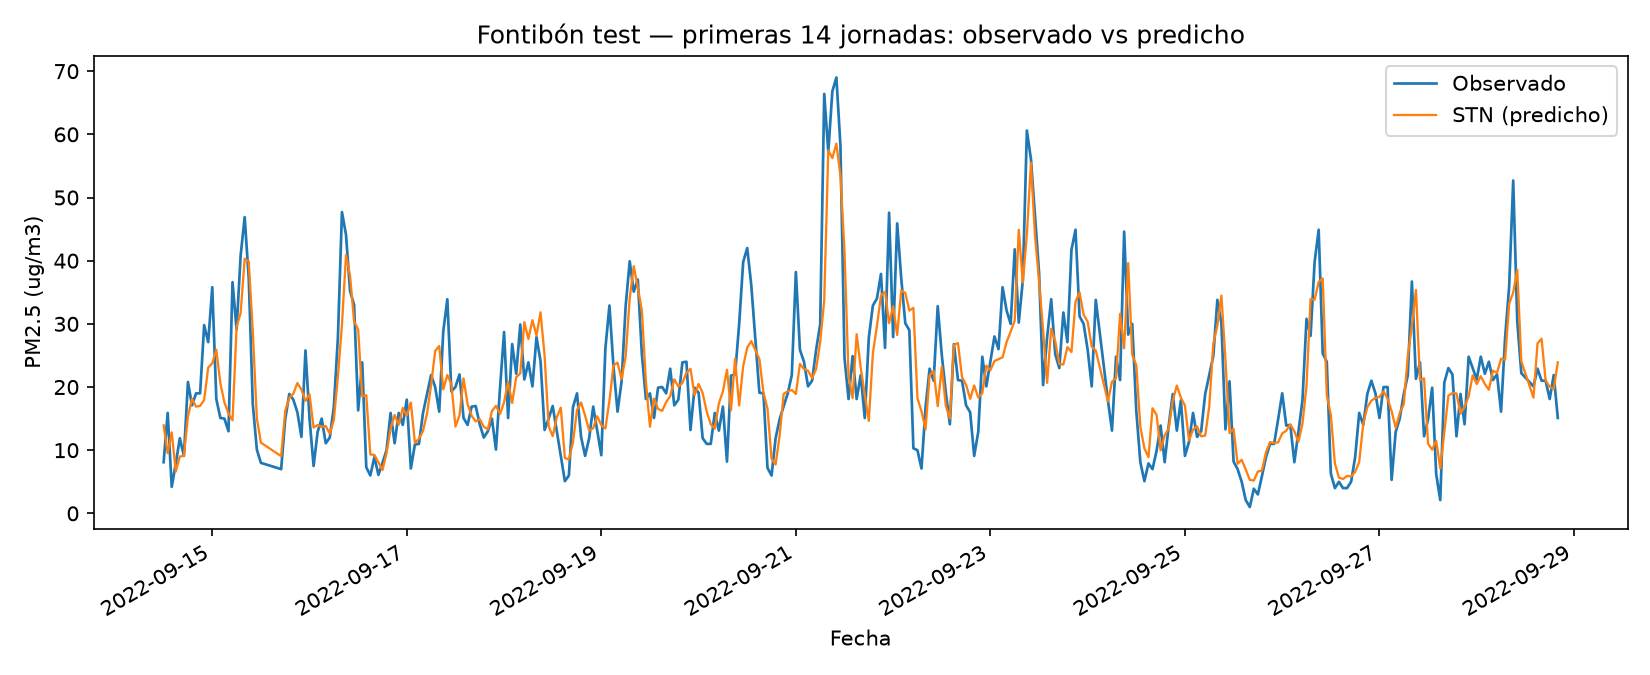
\includegraphics[width=\linewidth]{figuras/test_pred_vs_real.png}\caption{Primeras dos semanas de la prueba.}\end{subfigure}\hfill
\begin{subfigure}{0.32\textwidth}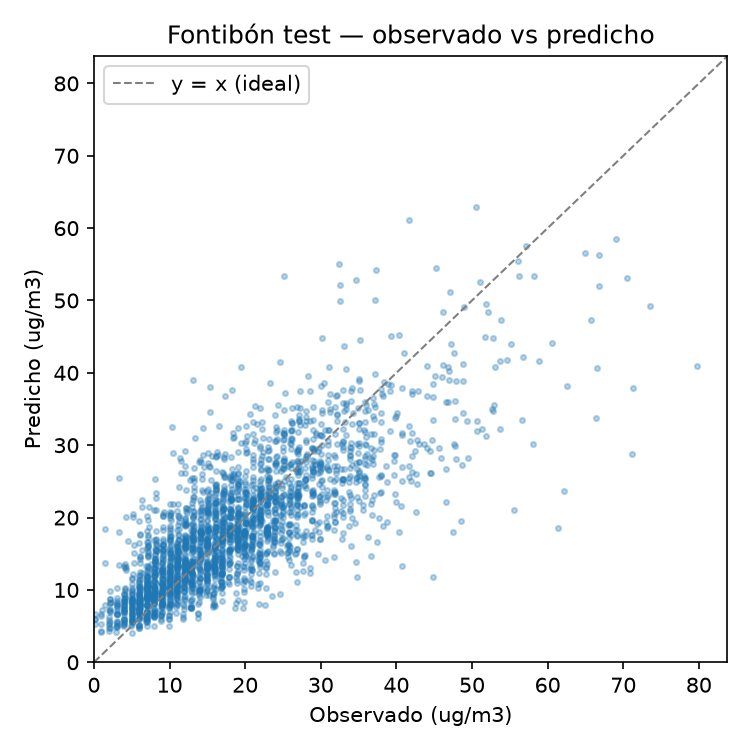
\includegraphics[width=\linewidth]{figuras/test_scatter.png}\caption{Real frente a predicho.}\end{subfigure}
\caption{Modelo A (semilla 42) en la prueba de Fontibón: sigue el nivel y el ciclo diario, pero llega tarde y corto a los picos.}
\label{fig:test}
\end{figure}

\begin{figure}[h]
\centering
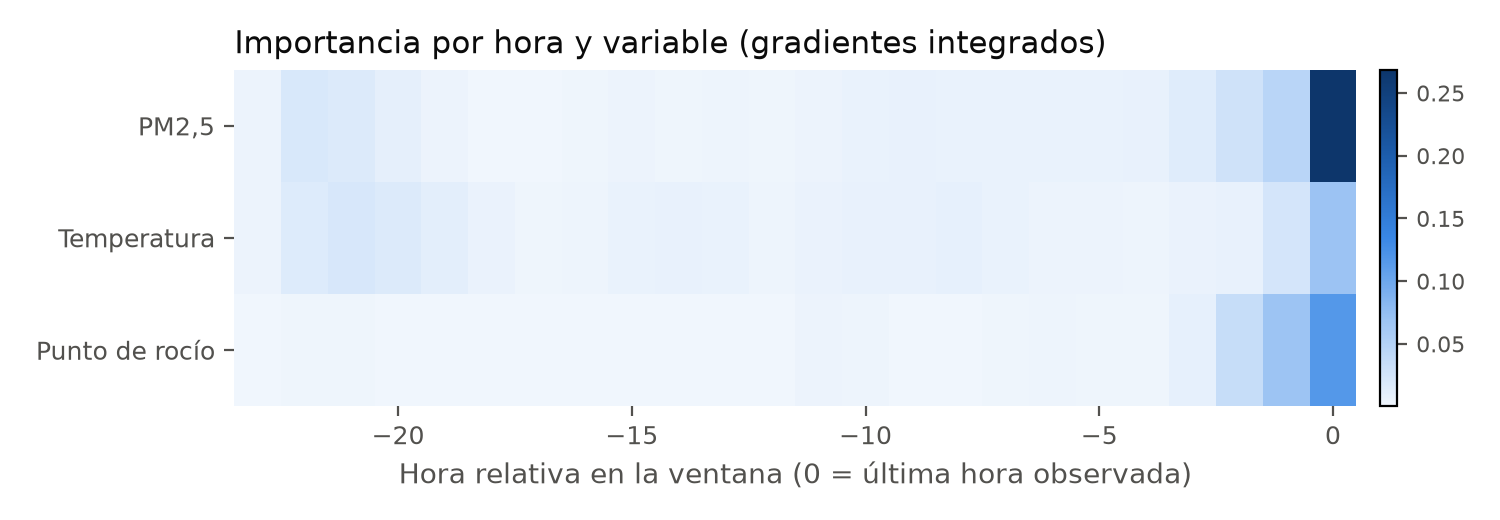
\includegraphics[width=0.85\textwidth]{figuras/ig_hora_variable.png}
\caption{Gradientes integrados: importancia por hora y variable (media de tres semillas, 518 ventanas). La atribución se concentra en las últimas horas de \PM{} y de meteorología.}
\label{fig:ig}
\end{figure}

\begin{figure}[h]
\centering
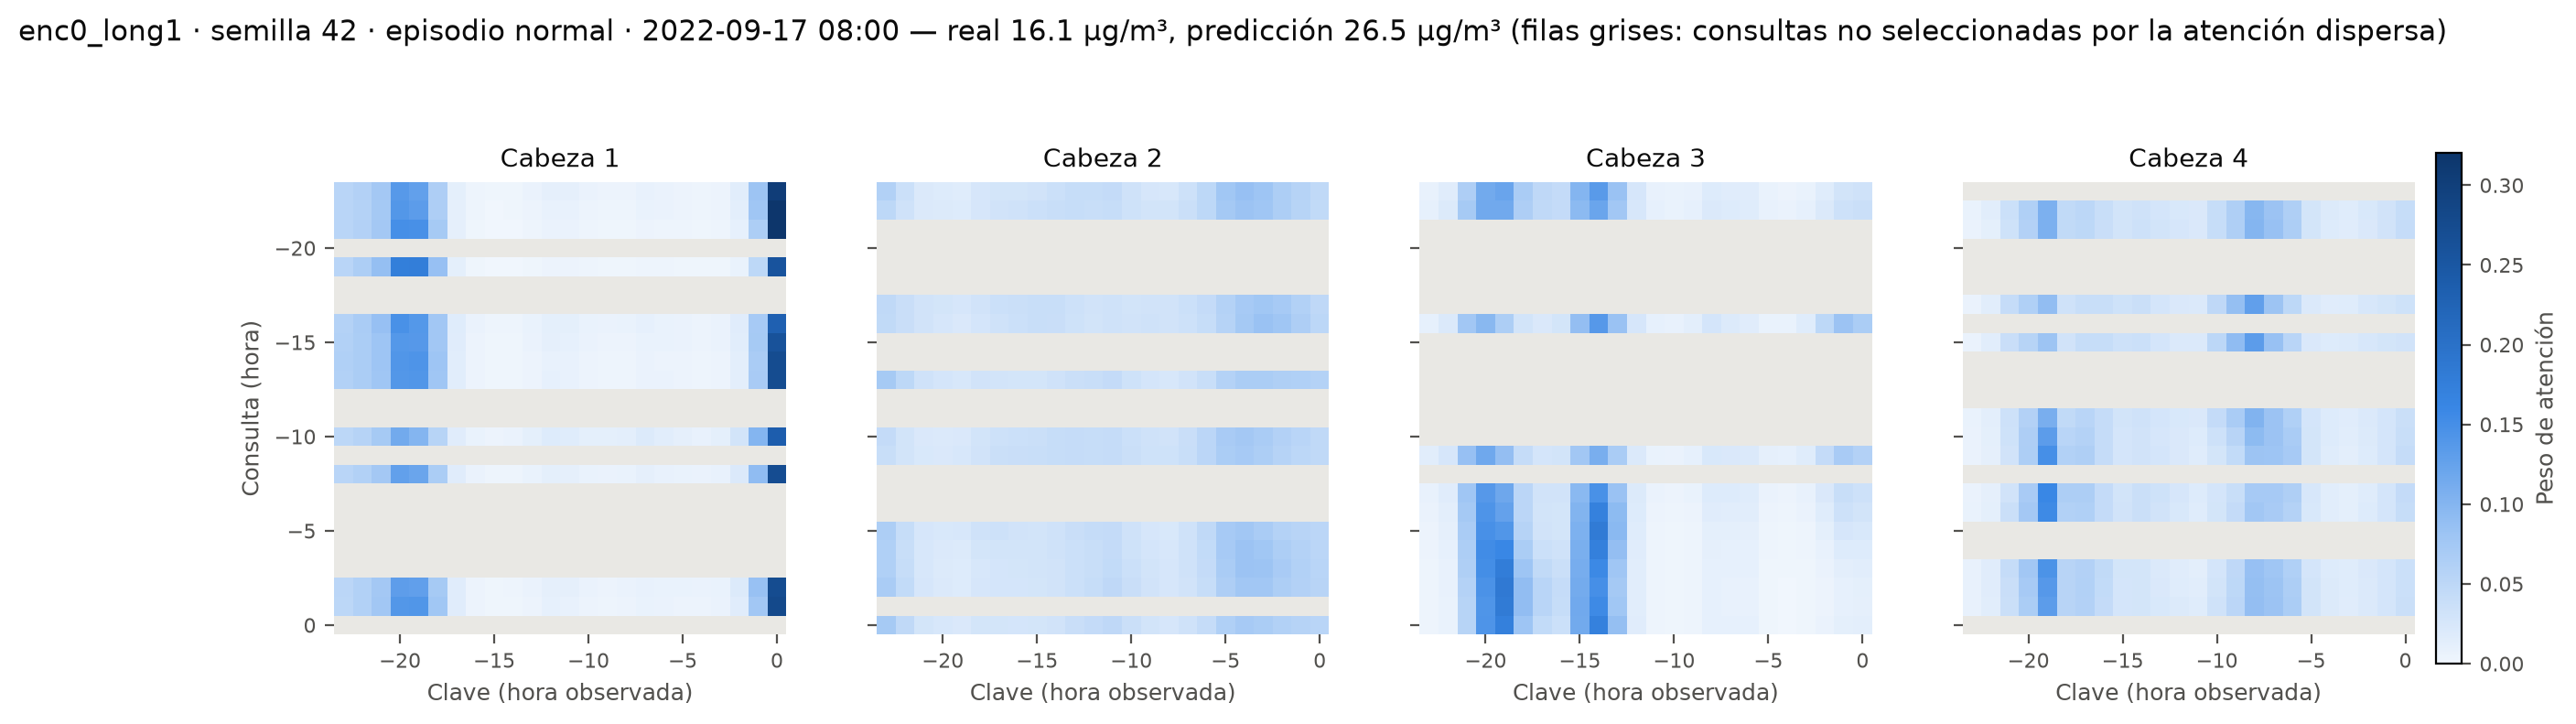
\includegraphics[width=\textwidth]{figuras/atencion_matriz_normal.png}\\[4pt]
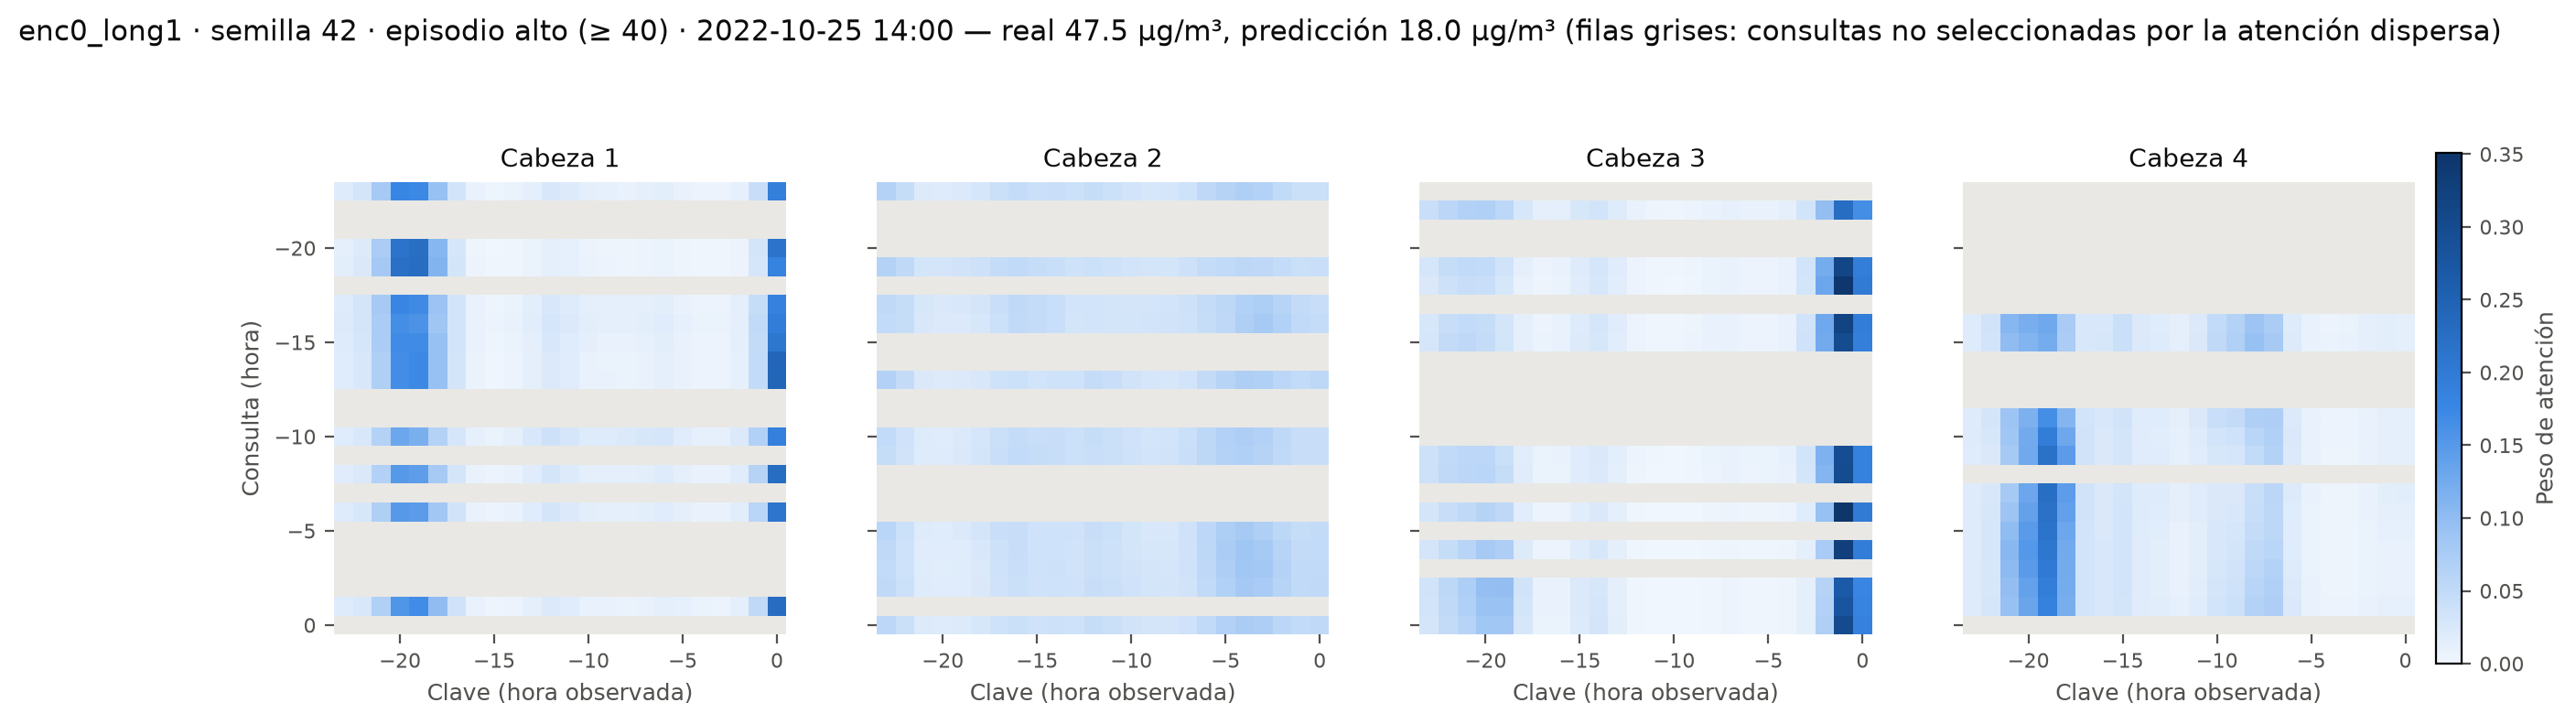
\includegraphics[width=\textwidth]{figuras/atencion_matriz_alto.png}
\caption{Matrices de atención consulta $\times$ clave de la primera capa del encoder (semilla 42), por cabeza y sin promediar. Arriba, episodio normal; abajo, episodio alto. Las filas grises son consultas no seleccionadas por la atención dispersa.}
\label{fig:mat}
\end{figure}

\begin{figure}[h]
\centering
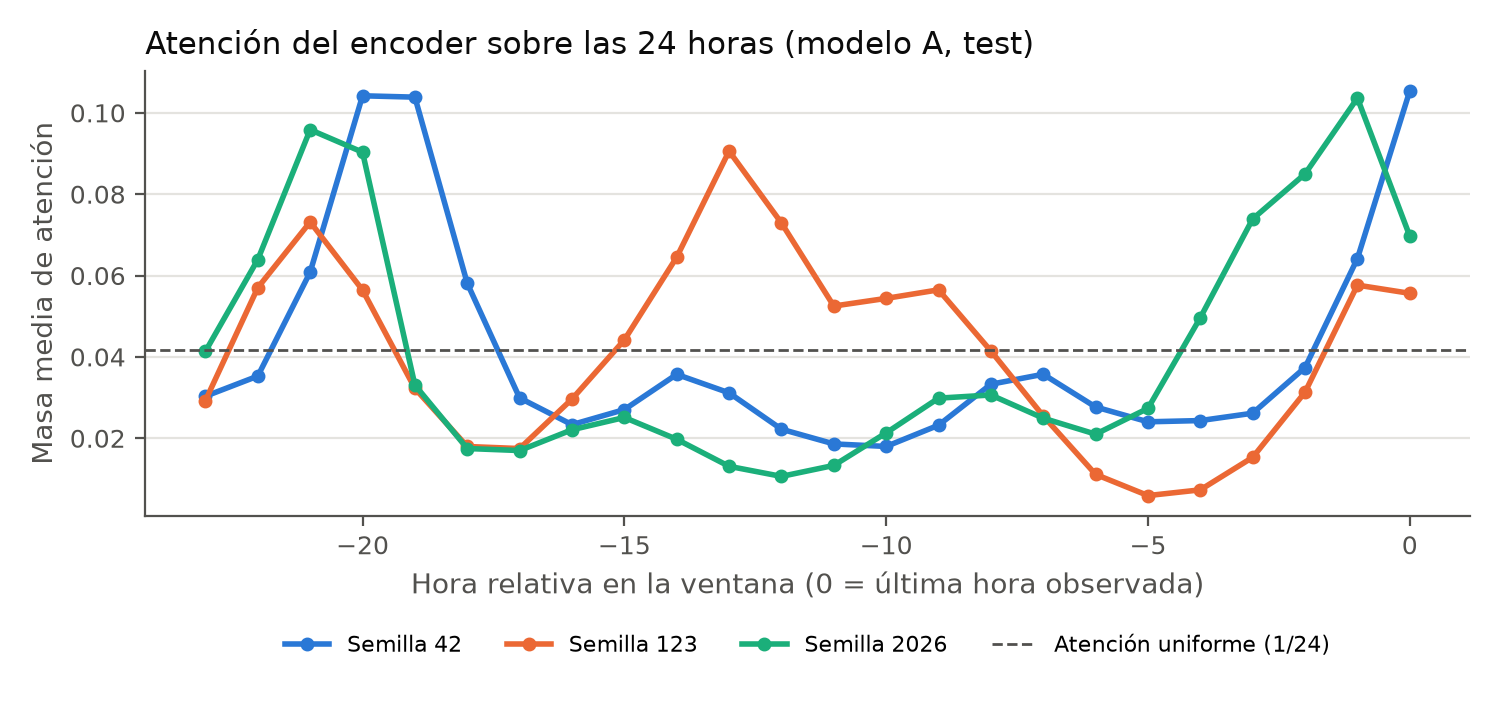
\includegraphics[width=0.85\textwidth]{figuras/atencion_por_hora.png}
\caption{Atención de la primera capa del encoder por hora y semilla. Con métricas casi idénticas, cada semilla distribuye la atención de forma distinta.}
\label{fig:att}
\end{figure}

\begin{figure}[h]
\centering
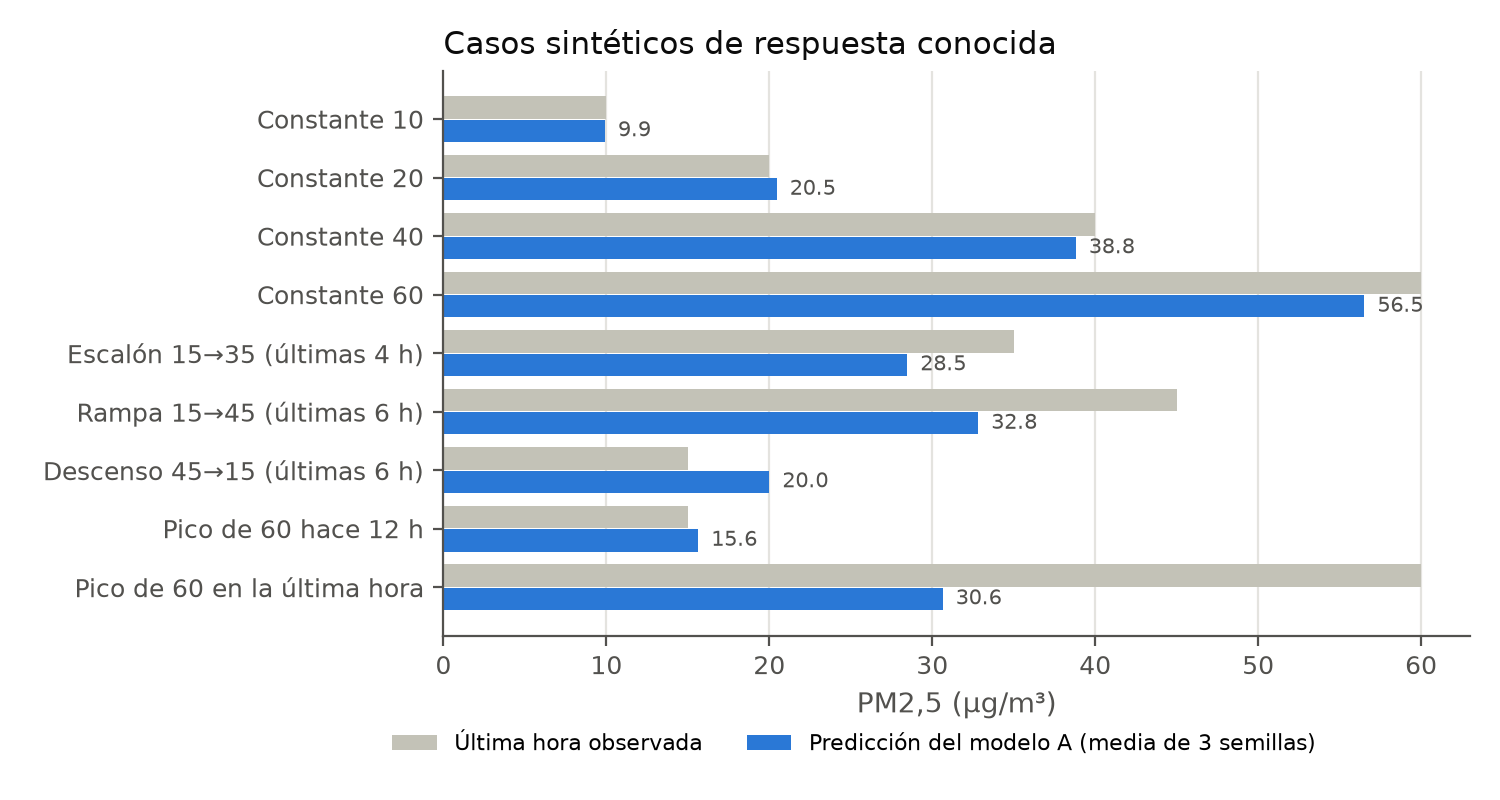
\includegraphics[width=0.78\textwidth]{figuras/casos_sinteticos.png}
\caption{Casos sintéticos de comportamiento esperado. Las series constantes se reproducen; los cambios recientes se amortiguan.}
\label{fig:sint}
\end{figure}

\begin{figure}[h]
\centering
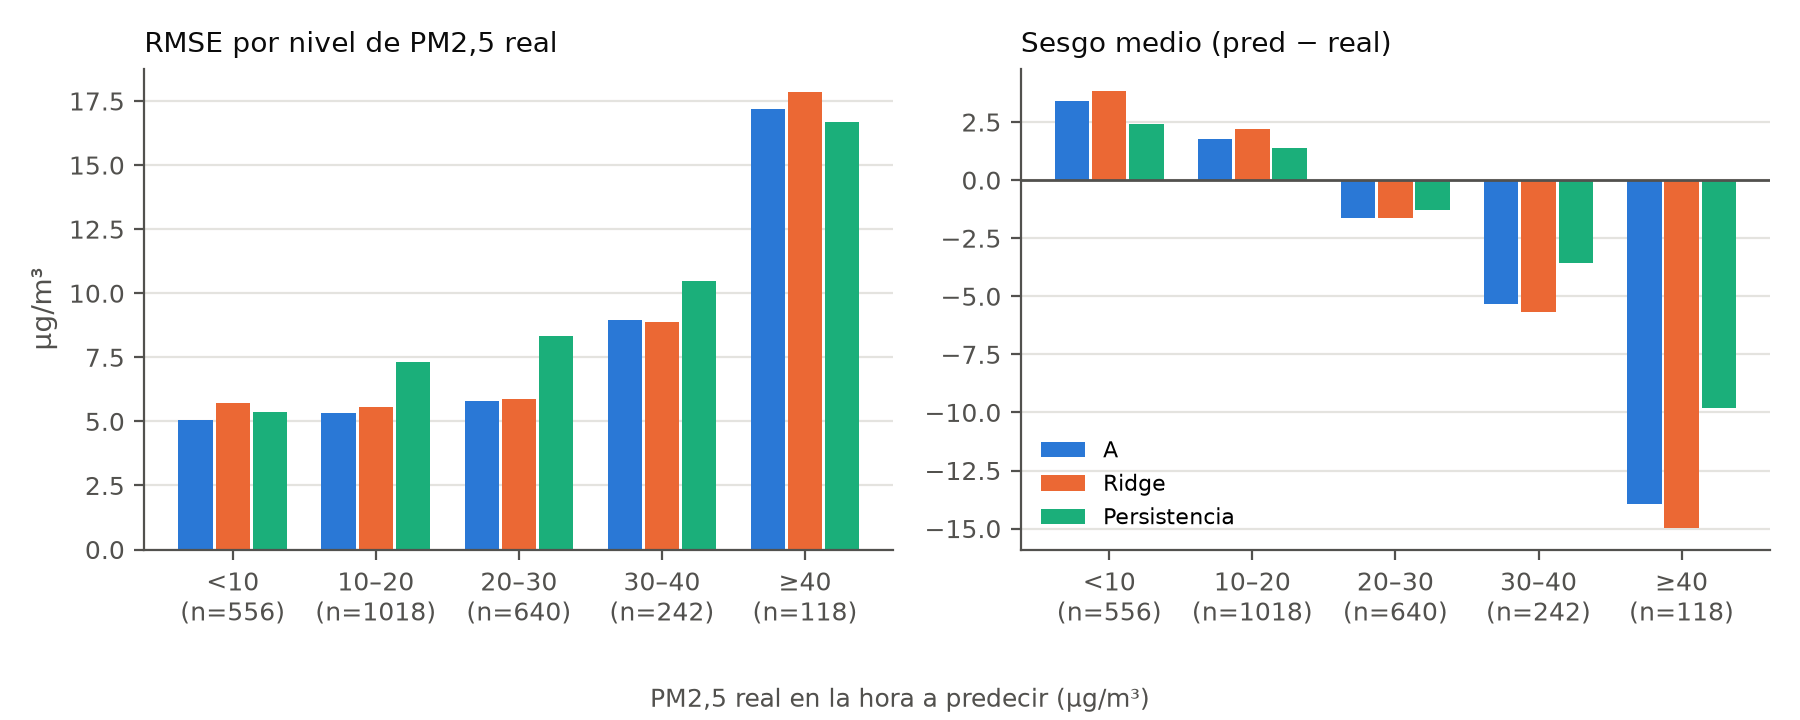
\includegraphics[width=0.95\textwidth]{figuras/error_por_nivel.png}
\caption{Error y sesgo por nivel de \PM{} real: los tres modelos sobreestiman el aire limpio y subestiman los episodios.}
\label{fig:nivel}
\end{figure}

\begin{figure}[h]
\centering
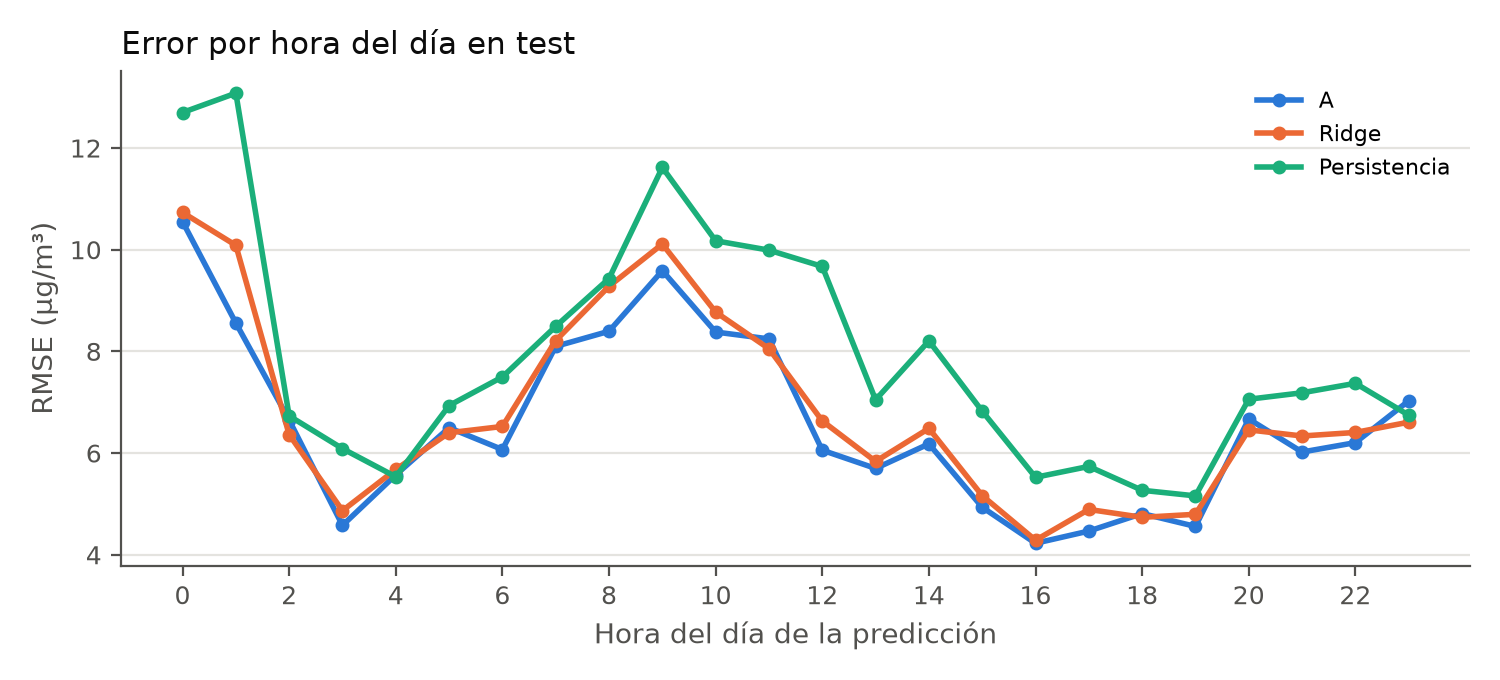
\includegraphics[width=0.8\textwidth]{figuras/error_por_hora.png}
\caption{Error por hora del día en la prueba: el máximo coincide con el pico de la mañana y con la medianoche.}
\label{fig:hora}
\end{figure}

\begin{figure}[h]
\centering
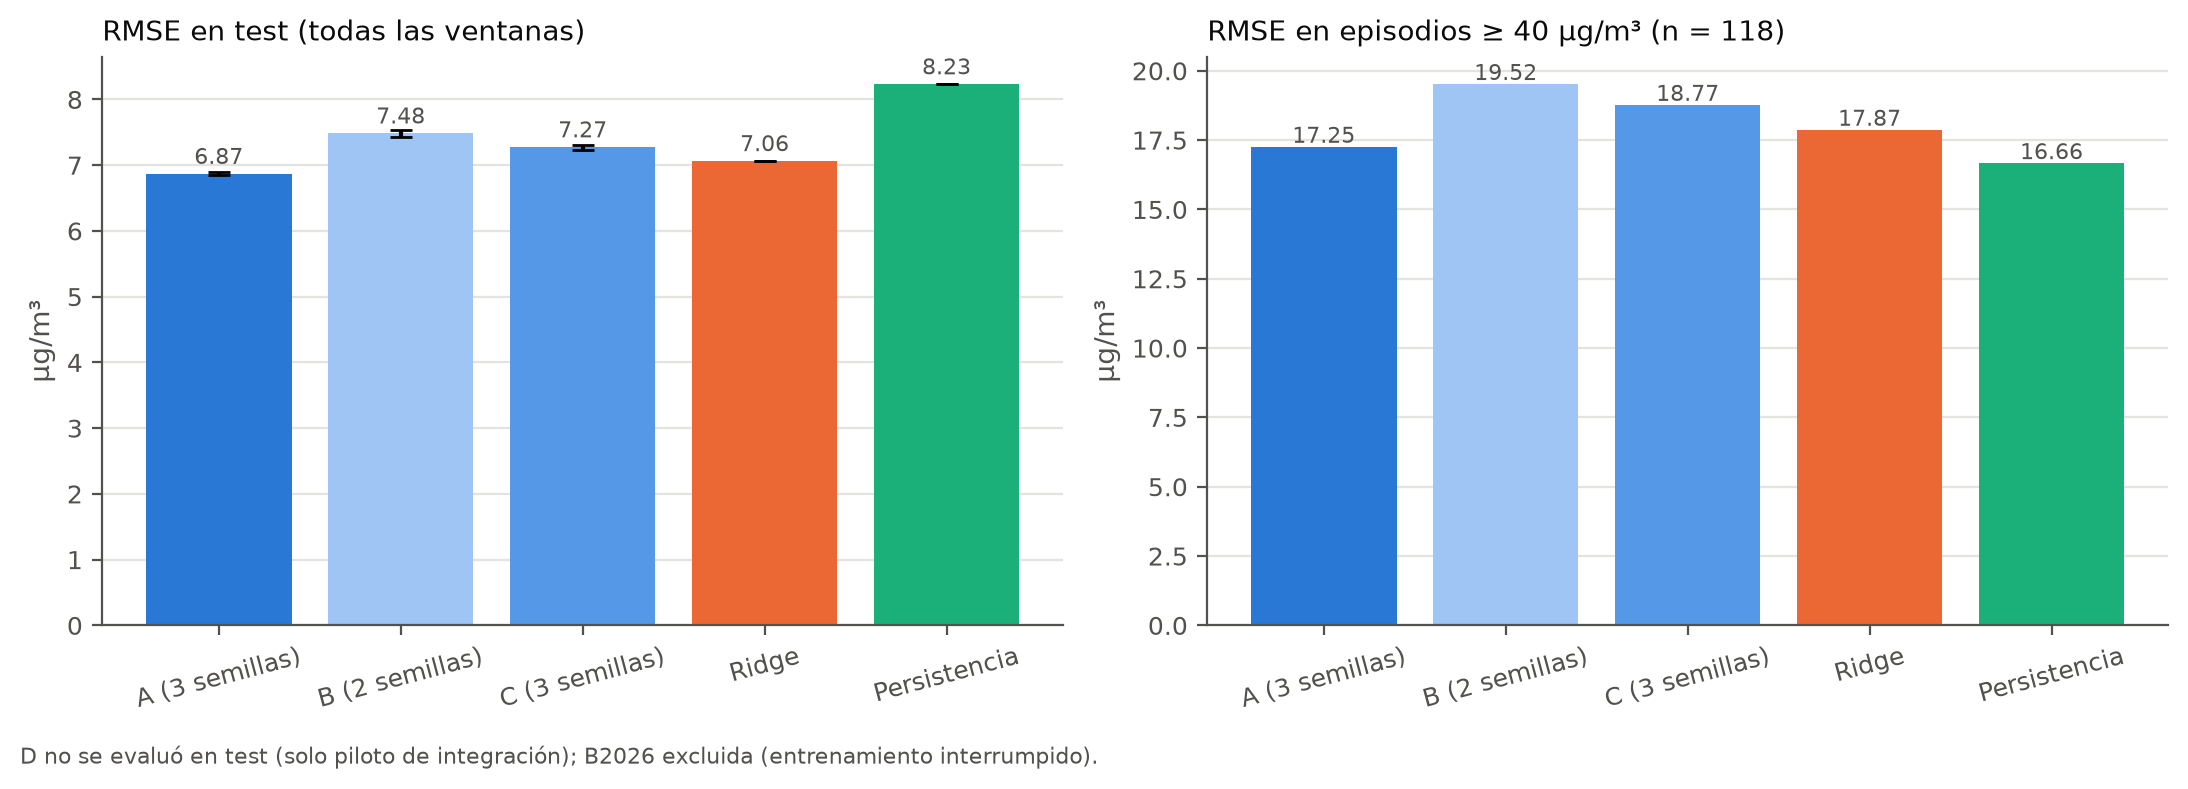
\includegraphics[width=0.95\textwidth]{figuras/comparacion_modelos.png}
\caption{RMSE en la prueba de todos los modelos evaluados. D no se evaluó (solo piloto de integración) y la tercera semilla de B se excluye por entrenamiento interrumpido.}
\label{fig:comp}
\end{figure}

\begin{figure}[h]
\centering
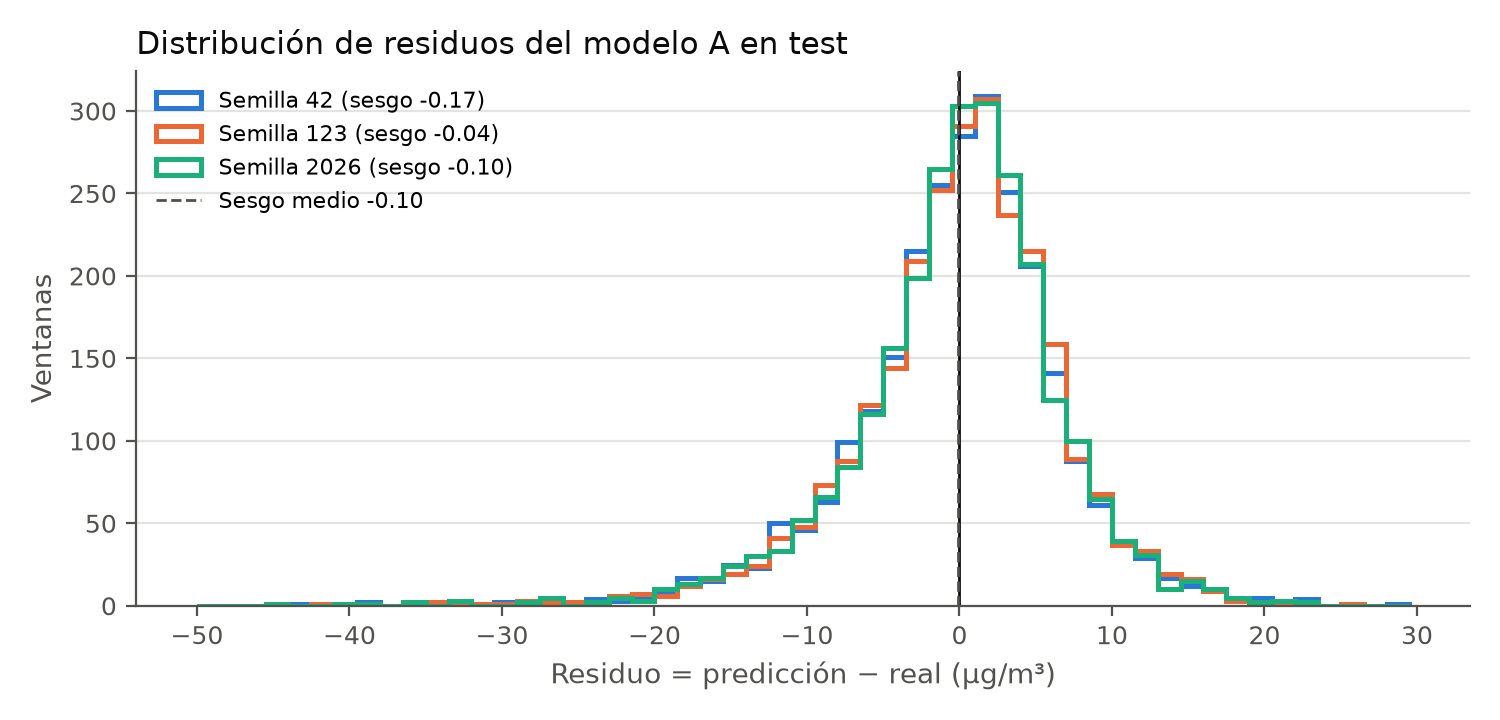
\includegraphics[width=0.75\textwidth]{figuras/residuos.png}
\caption{Distribución de residuos del modelo A en la prueba. La cola izquierda, más larga, corresponde a subestimaciones grandes en los episodios.}
\label{fig:res}
\end{figure}

% ------------------------------------------------------------------ cierre
\clearpage
\section*{Anexo A. Reproducibilidad, transparencia y uso de IA}

Este anexo está fuera del cuerpo principal del informe.

\textbf{Código reproducible:} anexo \texttt{EntregaFinal\_Codigo\_Reproducible.zip}.

\textbf{Entorno de referencia:} Python 3.12.10; las dependencias principales se encuentran fijadas en
\texttt{requirements.txt}.

Los resultados se generan con cinco scripts que no entrenan modelos y que se ejecutan en este orden:
\begin{enumerate}
\item \texttt{freeze\_f3\_protocol.py}: congela el protocolo antes de tocar la prueba.
\item \texttt{run\_f3\_test\_evaluation.py}: evaluación única; se niega a ejecutarse dos veces.
\item \texttt{run\_f3\_explainability.py}: explicabilidad; se ejecutó dos veces con resultados idénticos.
\item \texttt{run\_f3\_attention\_matrices.py}: matrices de atención y figuras de cierre; también se
  ejecutó dos veces con resultados idénticos.
\item \texttt{run\_f3\_failure\_analysis.py}: análisis de fallas.
\end{enumerate}
Las pruebas de integridad de esta fase están en \texttt{tests/test\_f3\_audit.py}.
Los resultados quedan en \texttt{outputs/metrics/F3\_*.json}, y el notebook \texttt{EntregaFinal\_DL.ipynb}
los lee sin recalcular. Como en la fase anterior, el archivo institucional de Fontibón y los checkpoints
no se incluyen en el paquete por su origen y tamaño.

\textbf{Declaración de uso de inteligencia artificial.} Se utilizaron herramientas de IA generativa como
apoyo en la programación de los scripts de auditoría, la organización de resultados y la redacción. Los
valores cuantitativos proceden de archivos de resultados obtenidos al ejecutar los experimentos; las
decisiones metodológicas y las conclusiones fueron revisadas por el integrante, quien debe poder
sustentarlas.

\section*{Referencias}
\small
\begin{enumerate}[label={[\arabic*]},leftmargin=2.2em]
\item Zhang, Z., \& Zhang, S. (2023). Modeling air quality PM2.5 forecasting using deep sparse attention-based transformer networks. \emph{International Journal of Environmental Science and Technology}, 20, 13535–13550. \url{https://doi.org/10.1007/s13762-023-04900-1}
\item Alfonso Albarracín, K. Y., Altamar Consuegra, A., \& Aguilar-Arias, J. (2023). Particulate matter 10\,$\mu$m (PM10), 2.5\,$\mu$m (PM2.5) datasets gathered by direct measurement, low-cost sensor and by public air quality stations in Fontibón, Bogotá D.C., Colombia. \emph{Data in Brief}, 49, 109323. \url{https://doi.org/10.1016/j.dib.2023.109323}
\item Chen, S. (2015). \emph{Beijing PM2.5} [Conjunto de datos]. UCI Machine Learning Repository. \url{https://doi.org/10.24432/C5JS49}
\item Zhou, H., et al. (2021). Informer: Beyond efficient transformer for long sequence time-series forecasting. \emph{Proceedings of the AAAI Conference on Artificial Intelligence}.
\item Vaswani, A., et al. (2017). Attention is all you need. \emph{Advances in Neural Information Processing Systems}, 30.
\item Jain, S., \& Wallace, B. C. (2019). Attention is not explanation. \emph{Proceedings of NAACL-HLT 2019}, 3543–3556.
\item Sundararajan, M., Taly, A., \& Yan, Q. (2017). Axiomatic attribution for deep networks. \emph{Proceedings of the 34th International Conference on Machine Learning}, 3319–3328.
\item Angelopoulos, A. N., \& Bates, S. (2023). Conformal prediction: A gentle introduction. \emph{Foundations and Trends in Machine Learning}, 16(4), 494–591.
\item Universidad Externado de Colombia. (2026). \emph{Guía del Proyecto Integrador: Deep Learning} [Documento del curso].
\end{enumerate}

\end{document}
